% Intended LaTeX compiler: pdflatex
\documentclass[a4paper]{memoir}
\usepackage{mathtools}
\makeatletter

\usepackage{vocabulary}

\def\maketitle{}

\makeatother

\setcounter{secnumdepth}{2}
\date{\today}
\title{Pāli Cheatsheet}
\hypersetup{
 pdfauthor={The Bhikkhu Saṅgha},
 pdftitle={Pāli Cheatsheet},
 pdfkeywords={},
 pdfsubject={},
 pdfcreator={Emacs 29.4 (Org mode 9.6.15)}, 
 pdflang={English}}
\begin{document}


\chapter{Pāli Cheatsheet}
\label{sec:orgd057acd}
\section{Masculine and Neuter Nouns Ending in -a}
\label{sec:org00f233c}

\begin{center}
\begin{tabular}{lllll}
 & \textbf{masc.sg.-a} & \textbf{nt.sg.-a} & \textbf{masc.pl.-a} & \textbf{nt.pl.-a}\\[0pt]
\hline
1. nom & nar\textbf{o} & citt\textbf{aṁ} & nar\textbf{ā} & citt\textbf{ā}, citt\textbf{āni}\\[0pt]
2. acc & nar\textbf{aṁ} & citt\textbf{aṁ} & nar\textbf{e} & citt\textbf{e}, citt\textbf{āni}\\[0pt]
3. inst & nar\textbf{ena} & citt\textbf{ena} & nar\textbf{ehi} & citt\textbf{ehi}\\[0pt]
4. dat & nar\textbf{āya}, nar\textbf{assa} & citt\textbf{āya}, citt\textbf{assa} & nar\textbf{ānaṁ} & citt\textbf{ānaṁ}\\[0pt]
5. abl & nar\textbf{ā}, nar\textbf{amhā}, nar\textbf{asmā} & citt\textbf{ā}, citt\textbf{amhā}, citt\textbf{asmā} & nar\textbf{ehi} & citt\textbf{ehi}\\[0pt]
6. gen & nar\textbf{assa} & citt\textbf{assa} & nar\textbf{ānaṁ} & citt\textbf{ānaṁ}\\[0pt]
7. loc & nar\textbf{e} nar\textbf{amhi} nar\textbf{asmiṁ} & citt\textbf{e} citt\textbf{amhi} citt\textbf{asmiṁ} & nar\textbf{esu} & citt\textbf{esu}\\[0pt]
8. voc & nar\textbf{a}, nar\textbf{ā} & citt\textbf{a} citt\textbf{ā} & nar\textbf{ā} & citt\textbf{āni}\\[0pt]
\end{tabular}
\end{center}

\section{Masculine and Neuter Nouns Ending in -u}
\label{sec:org3c7ff26}

\begin{center}
\begin{tabular}{lllll}
 & \textbf{masc.sg.} & \textbf{nt.sg.} & \textbf{masc.pl.} & \textbf{nt.pl.}\\[0pt]
\hline
1. nom & bhikkh\textbf{u} & āy\textbf{uṁ} & bhikkh\textbf{ū}, bhikkh\textbf{avo} & āy\textbf{ū}, āy\textbf{ūni}\\[0pt]
2. acc & bhikkh\textbf{uṁ} & āy\textbf{uṁ} & bhikkh\textbf{ū}, bhikkh\textbf{avo} & āy\textbf{ū}, āy\textbf{ūni}\\[0pt]
3. inst & bhikkh\textbf{unā} & āy\textbf{unā} & bhikkh\textbf{ūhi} & āy\textbf{ūhi}\\[0pt]
4. dat & bhikkh\textbf{uno}, bhikkh\textbf{ussa} & āy\textbf{uno}, āy\textbf{ussa} & bhikkh\textbf{ūnaṁ} & āy\textbf{ūnaṁ}\\[0pt]
5. abl & bhikkh\textbf{unā}, bhikkh\textbf{umhā}, & āy\textbf{unā}, āy\textbf{umhā}, & bhikkh\textbf{ūhi} & āy\textbf{ūhi}\\[0pt]
 & bhikkh\textbf{usmā} & āy\textbf{usmā} &  & \\[0pt]
6. gen & bhikkh\textbf{uno}, bhikkh\textbf{ussa} & āy\textbf{uno}, āy\textbf{ussa} & bhikkh\textbf{ūnaṁ} & āy\textbf{ūnaṁ}\\[0pt]
7. loc & bhikkh\textbf{umhi} bhikkh\textbf{usmiṁ} & āy\textbf{umhi} āy\textbf{usmiṁ} & bhikkh\textbf{ūsu} & āy\textbf{ūsu}\\[0pt]
8. voc & bhikkh\textbf{u} & āy\textbf{u} & bhikkh\textbf{ū}, bhikkh\textbf{avo}, & āy\textbf{ū}, āy\textbf{ūni}\\[0pt]
 &  &  & bhikkh\textbf{ave} & \\[0pt]
\end{tabular}
\end{center}

\textbf{masc.-i:} aggi → agg\textbf{ayo}

\textbf{masc.-ī:} pakkhī → pakkh\textbf{ino}

\textbf{nt.-i:} aṭṭhi → aṭṭh\textbf{īni}

\section{Feminine Nouns Ending in -ā and -i}
\label{sec:org96141ba}

\begin{center}
\begin{tabular}{lllll}
 & \textbf{fem.sg.-ā} & \textbf{fem.sg.-i} & \textbf{fem.pl.-ā} & \textbf{fem.pl.-i}\\[0pt]
\hline
1. nom & vedan\textbf{ā} & bhūm\textbf{i} & vedan\textbf{ā}, vedan\textbf{āyo} & bhūm\textbf{ī}, bhūm\textbf{iyo}\\[0pt]
2. acc & vedan\textbf{aṁ} & bhūm\textbf{iṁ} & vedan\textbf{ā}, vedan\textbf{āyo} & bhūm\textbf{ī}, bhūm\textbf{iyo}\\[0pt]
3. inst & vedan\textbf{āya} & bhūm\textbf{iyā} & vedan\textbf{āhi} & bhūm\textbf{īhi}\\[0pt]
4. dat & vedan\textbf{āya} & bhūm\textbf{iyā} & vedan\textbf{ānaṁ} & bhūm\textbf{īnaṁ}\\[0pt]
5. abl & vedan\textbf{āya} & bhūm\textbf{iyā} & vedan\textbf{āhi} & bhūm\textbf{īhi}\\[0pt]
6. gen & vedan\textbf{āya} & bhūm\textbf{iyā} & vedan\textbf{ānaṁ} & bhūm\textbf{īnaṁ}\\[0pt]
7. loc & vedan\textbf{āya}, vedan\textbf{āyaṁ} & bhūm\textbf{iyā}, bhūm\textbf{iyaṁ} & vedan\textbf{āsu} & bhūm\textbf{isu}, bhūm\textbf{īsu}\\[0pt]
8. voc & vedan\textbf{e} & bhūm\textbf{i} & vedan\textbf{ā}, vedan\textbf{āyo} & bhūm\textbf{ī}, bhūm\textbf{iyo}\\[0pt]
\end{tabular}
\end{center}

\textbf{fem.-ī:} kumārī → kumār\textbf{iyo}

\textbf{fem.-u:} yāgu → yāg\textbf{uyo}

\clearpage

\section{Simple Present}
\label{sec:org49ae9d4}

{\centering\par
\begin{multicols}{2}

Verbal terminations:

\begin{center}
\begin{tabular}{lll}
 & \textbf{sg.} & \textbf{pl.}\\[0pt]
\textbf{1st} & -mi & -ma\\[0pt]
\textbf{2nd} & -si & -tha\\[0pt]
\textbf{3rd} & -ti & -(a)nti\\[0pt]
\end{tabular}
\end{center}

The base is obtained by removing the 3rd.sg. termination \emph{-ti} from the conjugated form.

\columnbreak

Root: \emph{√dhāv} (to run), base: \emph{dhāva}

\begin{center}
\begin{tabular}{lll}
 & \textbf{sg.} & \textbf{pl.}\\[0pt]
\textbf{1st} & dhāvāmi & dhāvāma\\[0pt]
\textbf{2nd} & dhāvasi & dhāvatha\\[0pt]
\textbf{3rd} & dhāvati & dhāvanti\\[0pt]
\end{tabular}
\end{center}

The final \emph{-a} of the base is lengthened before \emph{m}: \emph{dhāvāmi, dhāvāma}.

\end{multicols}
\par}

\section{Future Tense}
\label{sec:org5ecbe86}

The verb \emph{atthi} (he is) is not used in the future tense, \emph{bhavissati} is used instead.

\begin{center}
\begin{tabular}{llll}
\textbf{sg.} &  & \textbf{pl.} & \\[0pt]
bhav\textbf{issāmi} & I will be & bhav\textbf{issāma} & we will be\\[0pt]
bhav\textbf{issasi} & you will be & bhav\textbf{issatha} & you all will be\\[0pt]
bhav\textbf{issati} & he will be & bhav\textbf{issanti} & they will be\\[0pt]
\end{tabular}
\end{center}

\section{Aorist Past Tense}
\label{sec:org98537e8}

{\centering\par
\begin{multicols}{2}

Verbal terminations:

\begin{center}
\begin{tabular}{lll}
 & \textbf{sg.} & \textbf{pl.}\\[0pt]
\textbf{1st} & -iṁ & -(i)mhā, -(i)mha\\[0pt]
\textbf{2nd} & -o, -i & -(i)ttha\\[0pt]
\textbf{3rd} & -i & -(i)ṁsu, -uṁ\\[0pt]
\end{tabular}
\end{center}

\columnbreak

Root: \emph{√dhāv} (to run), base: \emph{dhāva}

\begin{center}
\begin{tabular}{lll}
 & \textbf{sg.} & \textbf{pl.}\\[0pt]
\textbf{1st} & adhāviṁ & adhāvimhā\\[0pt]
\textbf{2nd} & adhāvo, adhāvi & adhāvittha\\[0pt]
\textbf{3rd} & adhāvi & adhāviṁsu, adhāvuṁ\\[0pt]
\end{tabular}
\end{center}

\end{multicols}
\par}

Bases ending in \textbf{e} are conjugated with an inserted ``s''.

\begin{center}
\begin{tabular}{lllll}
 & singular &  & plural & \\[0pt]
\hline
1st & dese\textbf{siṁ} & I taught & des\textbf{imha} & we taught\\[0pt]
 &  &  & des\textbf{imhā} & \\[0pt]
2nd & dese\textbf{si} & you taught & des\textbf{ittha} & you all taught\\[0pt]
3rd & dese\textbf{si} & he taught & dese\textbf{suṁ} & they taught\\[0pt]
\end{tabular}
\end{center}

Also applies to causative verbs (e.g. \emph{vandati} → \emph{vandāpeti} → \emph{vandāpesi}).

Similarly \emph{samacintesi, āmantesi, santappesi, samuttejesi} etc.

Some roots ending in long vowels also get the \emph{s} aorist ending. In the plural case, the long vowel is shortened.

\begin{center}
\begin{tabular}{lllll}
 & \textbf{sg.} &  & \textbf{pl.} & \\[0pt]
\hline
1st & aṭṭhā\textbf{siṁ} & I stood & aṭṭha\textbf{mha}, aṭṭha\textbf{mhā} & we stood\\[0pt]
2nd & aṭṭhā\textbf{si} & you stood & aṭṭha\textbf{ttha} & you all stood\\[0pt]
3rd & aṭṭhā\textbf{si} & he stood & aṭṭha\textbf{ṁsu} & they stood\\[0pt]
\end{tabular}
\end{center}

\clearpage

\section{Optative or Potential Verbs: May / Should (-eyya)}
\label{sec:org29d279f}

{\centering\par
\begin{multicols}{2}

Verbal terminations:

\begin{center}
\begin{tabular}{lll}
 & \textbf{sg.} & \textbf{pl.}\\[0pt]
\textbf{1st} & -eyyāmi, -emi & -eyyāma, -ema\\[0pt]
\textbf{2nd} & -eyyāsi, -esi & -eyyātha, -etha\\[0pt]
\textbf{3rd} & -eyya, -e & -eyyuṁ\\[0pt]
\end{tabular}
\end{center}

\columnbreak

Root: \emph{√dhāv} (to run), base: \emph{dhāva}

\begin{center}
\begin{tabular}{lll}
 & \textbf{sg.} & \textbf{pl.}\\[0pt]
\textbf{1st} & dhāveyyāmi, dhāvemi & dhāveyyāma, dhāvema\\[0pt]
\textbf{2nd} & dhāveyyāsi, dhāvesi & dhāveyyātha, dhāvetha\\[0pt]
\textbf{3rd} & dhāveyya, dhāve & dhāveyyuṁ\\[0pt]
\end{tabular}
\end{center}

\end{multicols}
\par}

{\centering\par
\begin{multicols}{2}

Irregular: \emph{√as} (to be), \emph{atthi}

\begin{center}
\begin{tabular}{lll}
 & \textbf{sg.} & \textbf{pl.}\\[0pt]
\textbf{1st} & siyaṁ, assaṁ & assāma\\[0pt]
\textbf{2nd} & siyā, assa & assatha\\[0pt]
\textbf{3rd} & siyā, assa & siyuṁ, assu, siyaṁsu\\[0pt]
\end{tabular}
\end{center}

\columnbreak

Irregular: \emph{√kar} (to do, make, work), \emph{karo}

\begin{center}
\begin{tabular}{lll}
 & \textbf{sg.} & \textbf{pl.}\\[0pt]
\textbf{1st} & kareyyāmi, kayirāmi & kareyyāma, kayirāma\\[0pt]
\textbf{2nd} & kareyyāsi, kayirāsi & kareyyātha, kayirātha\\[0pt]
\textbf{3rd} & kareyya, kayirā, kare & kareyyuṁ, kayiruṁ\\[0pt]
\end{tabular}
\end{center}

\end{multicols}
\par}

\section{Gerund (e.g. bhavitvā), a.k.a. Absolutive}
\label{sec:orgcb1f36d}

\begin{multicols}{2}

\begin{center}
\begin{tabular}{ll}
bhavati (is, becomes) & bhavitvā\\[0pt]
gacchati (goes) & gantvā\\[0pt]
labhati (gets, obtains) & labhitvā, laddhā\\[0pt]
deti / dadāti (gives) & datvā\\[0pt]
deseti (teaches) & desetvā\\[0pt]
\end{tabular}
\end{center}

\columnbreak

\begin{center}
\begin{tabular}{ll}
suṇāti (hears) & sutvā\\[0pt]
pivati (drinks) & pitvā\\[0pt]
passati (sees) & disvā\\[0pt]
jānāti (knows) & ñatvā / jānitvā\\[0pt]
karoti (does) & katvā\\[0pt]
\end{tabular}
\end{center}

\end{multicols}

\section{Infinitive (e.g. bhavituṁ)}
\label{sec:org3054727}

{\centering
\begin{multicols}{2}

\textbf{root + -tuṁ}

\begin{center}
\begin{tabular}{lll}
√dā & dātuṁ & to give\\[0pt]
√gam & ga\textbf{n}tuṁ & to go\\[0pt]
√han & hantuṁ & to kill\\[0pt]
√kar & k\textbf{ā}tuṁ & to do, to make\\[0pt]
√ñā & ñātuṁ & to know\\[0pt]
\end{tabular}
\end{center}

\columnbreak

\textbf{root + -ituṁ}

\begin{center}
\begin{tabular}{lll}
√car & carituṁ & to walk\\[0pt]
√jīv & jīvituṁ & to live\\[0pt]
√har & harituṁ & to carry\\[0pt]
√han & hanituṁ & to kill\\[0pt]
√pucch & pucchituṁ & to ask\\[0pt]
\end{tabular}
\end{center}

\end{multicols}
\par}

\section{Causative: Having It Done (-e, -aya, -āpe, -āpaya)}
\label{sec:orgca42151}

The causative base is formed by adding \emph{-e, -aya, -āpe, -āpaya} either to the root or the verbal base.
The base thus formed is conjugated in all tenses and moods. The causative form of a transitive verb takes two objects in the accusative.

\begin{multicols}{2}

vandati → vandāpeti → vandāpesi

\emph{Suppavāsā dārakaṁ Bhagavantaṁ vandāpesi.} \\[0pt]
Suppavāsā made her boy bow to the Blessed One.

\columnbreak

uggaṇhāti → uggahetvā → uggahāpetvā

\emph{\ldots{} uggahetvā vā uggahāpetvā vā nikkhipitabbaṁ.} \\[0pt]
\ldots{} having picked it up or causing it to be picked up, it should be kept.

\end{multicols}

\clearpage

\section{Present Participle (-nt, -māna)}
\label{sec:org9d2337c}

\begin{center}
\begin{tabular}{llll}
√gam & gaccha & gacchant, gacchamāna, gacchāna & going\\[0pt]
√dā & data & dadant, dadamāna, dadāna & giving\\[0pt]
√dis & dese & desent, desayamāna, desayāna & teaching\\[0pt]
√bhū & bhava & bhavanta & being\\[0pt]
\end{tabular}
\end{center}

{\centering

Irregular forms:

\par}

\begin{center}
\begin{tabular}{llll}
√as & sa & santa, samāna & being, existing\\[0pt]
√kar & karo & karont, karumāna, karāna & doing, making\\[0pt]
\end{tabular}
\end{center}

The present participles are declinable, they agree with the noun in gender, number and case.

\emph{gacchant → (nom.sg.) gacchaṁ, gacchanto (nom.pl) gacchanto, gacchantā}

\section{Future Passive Participle: Should Be Done (-tabba)}
\label{sec:org848ba79}

{\centering\par
\begin{multicols}{2}

\begin{center}
\begin{tabular}{lll}
√dā & dātabba, deyya & should be given\\[0pt]
√su & sotabba & should be listened to\\[0pt]
dese & desetabba & should be expounded\\[0pt]
\end{tabular}
\end{center}

\columnbreak

\begin{center}
\begin{tabular}{lll}
√kar & kātabba, karaṇīya & should be done\\[0pt]
√ñā & ñātabba, ñeyya & should be known\\[0pt]
√pā & peyya & should be drunk\\[0pt]
\end{tabular}
\end{center}

\end{multicols}
\par}

\section{Past Participle (-ta, -ita, -na)}
\label{sec:org06388ec}

Generally formed by adding \emph{-ta, -ita, -na} to the verbal root or base. Sandhi rules complicate the exact forms.

\begin{center}
\begin{tabular}{ll}
rukkho patito & the fallen tree\\[0pt]
antarāyiko dhammo vutto bhagavatā & said to be an obstacle by the Buddha\\[0pt]
Pubbe'bhinno mallako. & The cup is already broken.\\[0pt]
\end{tabular}
\end{center}

\null

\begin{center}
\begin{tabular}{lllll}
bhavati & √bhū & to be & bhūta & became\\[0pt]
passati & √dis & to see & di\textbf{ṭṭ}ha & seen\\[0pt]
gacchati & √gam & to go & gata & gone\\[0pt]
karoti & √kar & to do & kata & done\\[0pt]
labhati & √labh & to get & la\textbf{dd}ha & received\\[0pt]
jānāti & √ñā & to know & ñāta & known\\[0pt]
bhāsati & √bhās & to speak & bhāsita & spoken\\[0pt]
pabbajati & √vaj & to go on & pabbajita & ordained\\[0pt]
ṭhahati & √ṭhā & to stand & ṭhita & stood\\[0pt]
bhāveti & √bhū & bhāve & bhāvita & developed\\[0pt]
deseti & √dis & dese & desita & preached\\[0pt]
passati & √dis & passa & passita & seen\\[0pt]
vedayati & √vid & vedaya & vedayita & experienced\\[0pt]
chindati & √chid & to cut & chi\textbf{nn}a & cut\\[0pt]
khīyati & √khī & to destroy & khīna & destroyed\\[0pt]
nisīdati & √sad & to sink & nisi\textbf{nn}a & seated\\[0pt]
pajahati & √hā & to abandon & pah\textbf{ī}na & abandoned\\[0pt]
\end{tabular}
\end{center}

\clearpage

\section{Irregular verb √as (to be)}
\label{sec:orgd680142}

{\centering\par
\begin{multicols}{3}

Present Tense

\begin{center}
\begin{tabular}{lll}
 & \textbf{sg.} & \textbf{pl.}\\[0pt]
\hline
1st & amhi & amha\\[0pt]
 & asmi & amhā\\[0pt]
 &  & asma\\[0pt]
2nd & asi & attha\\[0pt]
3rd & atthi & santi\\[0pt]
\end{tabular}
\end{center}

\columnbreak

Imperative Mood

\begin{center}
\begin{tabular}{lll}
 & \textbf{sg.} & \textbf{pl.}\\[0pt]
\hline
1st & amhi & amha\\[0pt]
 & asmi & amhā\\[0pt]
 &  & asma\\[0pt]
2nd & āhi & attha\\[0pt]
3rd & atthu & santu\\[0pt]
\end{tabular}
\end{center}

\columnbreak

Aorist Past Tense

\begin{center}
\begin{tabular}{lll}
 & \textbf{sg.} & \textbf{pl.}\\[0pt]
\hline
1st & ās\textbf{iṁ} & ās\textbf{imha}\\[0pt]
 &  & ās\textbf{imhā}\\[0pt]
2nd & ās\textbf{i} & ās\textbf{ittha}\\[0pt]
3rd & ās\textbf{i} & ās\textbf{iṁsu}\\[0pt]
 &  & ās\textbf{uṁ}\\[0pt]
\end{tabular}
\end{center}

\end{multicols}
\par}

\section{Irregular verb √hū (to be)}
\label{sec:orgd89c620}

{\centering\par
\begin{multicols}{3}

Present Tense

\begin{center}
\begin{tabular}{lll}
 & \textbf{sg.} & \textbf{pl.}\\[0pt]
\hline
1st & homi & homa\\[0pt]
2nd & hosi & hotha\\[0pt]
3rd & hoti & honti\\[0pt]
\end{tabular}
\end{center}

\columnbreak

Imperative Mood

\begin{center}
\begin{tabular}{lll}
 & \textbf{sg.} & \textbf{pl.}\\[0pt]
\hline
1st & homi & homa\\[0pt]
2nd & hohi & hotha\\[0pt]
3rd & hotu & hontu\\[0pt]
\end{tabular}
\end{center}

\columnbreak

Aorist Past Tense

\begin{center}
\begin{tabular}{lll}
 & \textbf{sg.} & \textbf{pl.}\\[0pt]
\hline
1st & ahos\textbf{iṁ} & ahu\textbf{mhā}\\[0pt]
 &  & ahu\textbf{mha}\\[0pt]
2nd & ahos\textbf{i} & ahuva\textbf{ttha}\\[0pt]
3rd & ahos\textbf{i} & ahes\textbf{uṁ}\\[0pt]
\end{tabular}
\end{center}

\end{multicols}
\par}

\section{Pronouns}
\label{sec:org6fde3ec}

{\centering\par
\begin{multicols}{2}

Personal pronouns (nominative)

\begin{center}
\begin{tabular}{lll}
 & \textbf{sg.} & \textbf{pl.}\\[0pt]
\textbf{1st} & ahaṁ & amhe, mayaṁ, no\\[0pt]
\textbf{2nd} & tuvaṁ, tvaṁ & tumhe, vo\\[0pt]
\textbf{3rd.masc.} & so, sa & te\\[0pt]
\textbf{3rd.nt.} & taṁ, tad & tāni\\[0pt]
\textbf{3rd.fem.} & sā & tā, tāyo\\[0pt]
\end{tabular}
\end{center}

\columnbreak

Possessive pronouns (genitive)

\begin{center}
\begin{tabular}{ll}
\textbf{sg.} & \textbf{pl.}\\[0pt]
mama, mayhaṁ, me & amhākaṁ, no\\[0pt]
tava, tuyhaṁ, te & tumhākam\\[0pt]
tassa & tesaṁ\\[0pt]
tassa & tesaṁ\\[0pt]
tassā & tāsaṁ\\[0pt]
\end{tabular}
\end{center}

\end{multicols}
\par}

\begin{center}
\begin{tabular}{lll}
ta → & \emph{(nom.sg.)} so / taṁ / sā & \emph{(nom.pl.)} te / tāni / tā, tāyo\\[0pt]
 & \emph{(acc.sg.)} taṁ & \emph{(acc.pl.)}  te / tāni / tā, tāyo\\[0pt]
\end{tabular}
\end{center}

\section{Compounds of Nouns Overview}
\label{sec:org995a596}

\hspace{-20pt}%
\begin{minipage}{\linewidth+10pt}%

\begin{longtable}{llll}
\textbf{Tappurisa} & \textbf{Kammadhāraya} & \textbf{Dvanda} & \textbf{Bahubbīhi}\\[0pt]
expresses: & \emph{A} is an \textbf{attribute} of \emph{B} & \textbf{List} & \emph{AB} is a \textbf{quality} of \emph{C}\\[0pt]
\emph{A} has \textbf{case-relation} to \emph{B} & \emph{A} is \textbf{equivalent} to \emph{B} &  & \emph{AB} → obj. outside of the comp.\\[0pt]
\hline
\endfirsthead
\multicolumn{4}{l}{Continued from previous page} \\[0pt]

\emph{A} has \textbf{case-relation} to \emph{B} & \emph{A} is \textbf{equivalent} to \emph{B} &  & \emph{AB} → obj. outside of the comp. \\[0pt]

\hline
\endhead
\hline\multicolumn{4}{r}{Continued on next page} \\
\endfoot
\endlastfoot
\hline
\(A \xrightarrow{\text{case}} B\) & an \emph{A}-like \emph{B} & \(A \mathbin{\&} B\) & \([A B] \rightarrow C\)\\[0pt]
 & an \emph{A} that is \emph{B} &  & \\[0pt]
\hline
\textbf{Case relation:} any except nom. voc. & \emph{A} \emph{B} in same case & \emph{A} \emph{B} in same case & case depends on \([A B]\)\\[0pt]
\hline
\hline
\emph{brahma-loko} & \emph{mahā-nadī} & \emph{samaṇa-brāhmaṇā} & \emph{su-desito dhammo}\\[0pt]
\(A \xrightarrow{\text{gen}} B\) & \(A_{\text{adj}} B_{\text{sub}}\) &  & \(A_{\text{adj}} B_{\text{sub}} \rightarrow C\)\\[0pt]
world \emph{of} Brahma & great river & recluses \& priests & the well-taught doctrine\\[0pt]
 &  &  & \\[0pt]
\hline
\emph{arañña-vāso} & \emph{sabba-seta} & \emph{nāma-rūpaṁ} & \emph{brāhmaṇo chinna-kukkucco}\\[0pt]
\(A \xrightarrow{\text{loc}} B\) & \(A_{\text{adj}} B_{\text{adj}}\) &  & \(C \leftarrow A_{\text{adj}} B_{\text{sub}}\)\\[0pt]
living \emph{in} forest & all white & name \& form & a brahmin (whose) worries (are) cut\\[0pt]
 &  &  & \\[0pt]
\hline
\emph{rukkha-patito} & \emph{mano-seṭṭha} & \emph{jarā-maraṇaṁ} & \emph{buddha-bhāsito dhammo}\\[0pt]
\(A \xrightarrow{\text{abl}} B\) & \(A_{\text{sub}} B_{\text{adj}}\) &  & \(A_{\text{sub}} B_{\text{adj}} \rightarrow C\)\\[0pt]
fallen \emph{from} tree & mind as foremost & old age \& death & the Buddha-spoken doctrine\\[0pt]
 &  &  & \\[0pt]
\hline
\emph{saraṇa-gamanaṁ} & \emph{sāriputta-thera} & \emph{hattha-pādaṁ} & \emph{kām'-andho puriso}\\[0pt]
\(A \xrightarrow{\text{acc}} B\) & \(A_{\text{sub}} B_{\text{sub}}\) &  & \(A_{\text{sub}} B_{\text{adj}} \rightarrow C\)\\[0pt]
going \emph{for} refuge & Sāriputta, the elder & hands \& feet & a desire-blinded man\\[0pt]
 &  &  & \\[0pt]
\hline
\emph{kūṭāgārasālā} & \emph{mukha-canda} & \emph{candima-suriyā} & \emph{pīti-sukhaṁ paṭhamaṁ jhānaṁ}\\[0pt]
\(A \xrightarrow{\text{gen}} B \xrightarrow{\text{gen}} C\) & \(A_{\text{sub}} B_{\text{sub}}\) &  & \(A \mathbin{\&} B \rightarrow C\)\\[0pt]
hall \emph{of} house \emph{with} a ridge & moon-like face & moon \& sun & the 1st jhāna (that is) joy \& ease\\[0pt]
 &  &  & \\[0pt]
\hline
\hline
\textbf{Avyayībhāva} &  & \textbf{Digu} & sub-type of\\[0pt]
Adverbial &  & Numerical & \emph{kammadhāraya}\\[0pt]
\hline
adv. don't take a case &  & \emph{A} \emph{B} in same case & \\[0pt]
\hline
\(A_{\text{prefix}} B_{\text{noun}}\) & \(A_{\text{ind}} B_{\text{noun}}\) & \(A_{\text{num}} B\) (sg.nt.) & \(A_{\text{num}} B\) (not nt.)\\[0pt]
\emph{paṭisotaṁ} & \emph{yathābhūtaṁ} & \emph{sattāhaṁ} & \emph{ekapuggalo}\\[0pt]
against the stream & as it is & seven days & one person\\[0pt]
\emph{nimmakasaṁ} & \emph{yāvajīvaṁ} & \emph{saḷāyatanaṁ} & \emph{tibhavā}\\[0pt]
mosquito-free & for the length of life & six senses & three spheres of existence\\[0pt]
\emph{ajjhattaṁ} [adhi + atta] & \emph{pacchābhattaṁ} & \emph{ticīvaraṁ} & \emph{catuddisā}\\[0pt]
inner; personal; subjective & after the meal & three robes & four directions\\[0pt]
\end{longtable}

\end{minipage}

\clearpage

\section{Declension Cases Overview}
\label{sec:org599f98f}

\casesLegendHeaderBGHere

\begin{tabular}{lll}
1. Nominative & subject performing the action & Who is giving?\\[0pt]
2. Accusative & direct object & What is he/she giving?\\[0pt]
3. Instrumental & means, instrument & With/by/through what?\\[0pt]
4. Dative & indirect object, recipient, purpose & To whom? For what?\\[0pt]
5. Ablative & motion/separation from, comparison & From where? Better than what?\\[0pt]
6. Genitive & possession, relationship & Whose?\\[0pt]
7. Locative & location, time & Where?\\[0pt]
8. Vocative & direct address & Form, bhikkhus, is not-self.\\[0pt]
\end{tabular}

\bigskip {\centering
Mnemonics:
\par}

\begin{center}
\begin{tabular}{ll}
1. \textbf{Nominate} who will do it. & 5. Pieces fall from the \textbf{ablative} heat-shield.\\[0pt]
2. Give an objective \textbf{accusation}. & 6. The \textbf{genitive} glues possessions to people.\\[0pt]
3. Fix it with this \textbf{instrument}. & 7. \textbf{Locate} him in space and time.\\[0pt]
4. \textbf{Donate} a date to him. & 8. Shout a \textbf{vocal} address.\\[0pt]
\end{tabular}
\end{center}

Origin of the word ``Dative'':

\begin{center}
\begin{tabular}{ll}
PIE root: & \emph{√do-} to give\\[0pt]
Latin: & \emph{donum} gift, \emph{donatio} a giving, \emph{dativus} pertaining to giving\\[0pt]
Pāli/Sanskrit: & \emph{dadāti} gives [√dā + dā + a → dadā]\\[0pt]
\end{tabular}
\end{center}

Origin of the word ``Ablative'':

\begin{center}
\begin{tabular}{lllll}
Latin & PIE & Pāli/Sanskrit &  & \\[0pt]
\emph{ab-} & \emph{√apo} & \emph{apa-} & off, away from & apocalypse, apology, apostle\\[0pt]
\emph{ferre} & \emph{√bher-} & \emph{√bhar} / \emph{√bhṛ} & to carry, to bear & birth, bring, burden,\\[0pt]
 &  &  &  & differ, offer, suffer, transfer\\[0pt]
\end{tabular}
\end{center}

\bigskip

{\centering
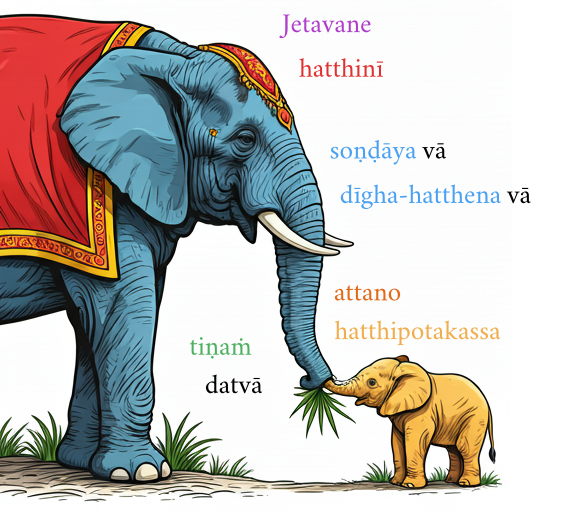
\includegraphics[width=0.5\linewidth]{./images/jetavane-hatthini.png}%
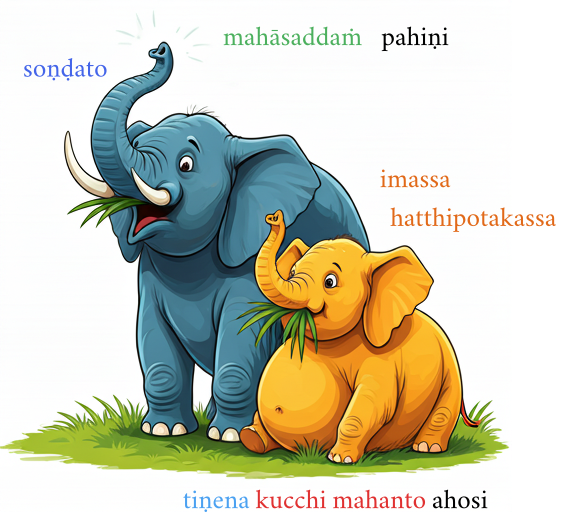
\includegraphics[width=0.5\linewidth]{./images/sondato-mahasaddam-pahini.png}%
\par}
\end{document}
